\documentclass[Proceedings]{ascelike}
%
% Feb. 14, 2013
%
% Some useful packages...
%
\usepackage{graphicx} \usepackage{float}
%\usepackage{cite}
\usepackage{cleveref}
%\usepackage{subfigure} \usepackage{amsmath} \usepackage{amsfonts}
%\usepackage{amssymb} \usepackage{amsbsy} \usepackage{times}
%
%
% Place hyperlinks within the pdf file (works only with pdflatex, not latex)
% \usepackage[colorlinks=true,citecolor=red,linkcolor=black]{hyperref}
%
%
% NOTE: Don't include the \NameTag{<your name>} if you have selected the
% NoPageNumbers option: this leads to an inconsistency and a warning, and the
% NameTag is ignored.
%
%
\begin{document}
%
% You will need to make the title all-caps
\title{Neural Network Initialization}
%
\author{ Vivek Rathod, Guifan Li }
%
\maketitle
%

\Section{Abstract} This report describes the results of experiments we
performed for the Neural Network weight Initialization project.

\Section{1. Network Structure} \label{sec:network_struct} We built a
shallow feed forward neural network with one hidden layer with $tanh$
activation units as recommended in \cite{lecun2012efficient}
\[1.7159*\tanh\left(\frac{2}{3}x\right)\] and an output layer with $softmax$
activation units to model the problem as a multinomial classification
problem:\[P(y=j|x)=\frac{e^{x^{T}w_j}}{\sum_{k=1}^Ke^{x^{T}w_k}}\] The input
layer has $784$ units and the output layer has $10$ units corresponding to the
ten target classes.

\Section{2. Training method} \label{sec:train_method} The neural network is
trained using mini-batch stochastic gradient descent (SGD) and back propagation
with a batch size of $32$. A constant learning rate of $0.01$ is used. No
regularization is applied. SGD is run for a fixed number of iterations and the
model that performs best on the validation set at any time during training is
used as the final model. 

\Section{3. Weight Initialization} \label{sec:weight_init} Neural Networks are
commonly initialized with weights sampled randomly from a uniform distribution
such that the network begins operating in its linear regime. This ensures that
the gradients are large enough when the training begins. In addition, it also
helps the network to learn the linear features first and harder non-linear
features later. Weights at each layer are initialized using the following
heuristic: \[W_{ij} = U\left[-\frac{1}{\sqrt{n}},\frac{1}{\sqrt{n}}\right]\]
where $U[-a, a]$ is the uniform distribution in the interval $(-a, a)$ and $n$
is the size of the previous layer ~\cite{erhan2009difficulty}. The biases are
set to zero.

\Section{4. Experiments} The mnist training data set is split into two: one set of
$50000$ examples is used for training and the set of other $10000$ examples is
used for the validation. The standard mnist test set is used for testing the
performance of the neural network. The dataset is standardized to have a mean
of zero and variance of one in all features.  \subsection{Shallow Neural
Network} We set up a shallow neural network as described in
section~\ref{sec:network_struct} with $300$ hidden units. The weights were
initialized as described in section~\ref{sec:weight_init}. The network was
trained with mini-batch SGD back propagation. The network achieves zero
training error after $30$ passes through the dataset and it achieves an error
of $3.6\%$ on the test set. The Training and Validation errors over training
epochs are show in figure~\ref{fig:sn_test_err}. We also plot the distribution
of weights and biases to  monitor the change during training in
figure~\ref{fig:wt_dist}.  We observe that the magnitude of the weights and
biases of layer $2$ (weights mapping the hidden layer to output layer) are
larger than the weights and biases of layer $1$(weights mapping the input layer to the
hidden layer).  Also, the gradients of the cost function calculated at each
layer decrease in the direction from output to input layer.  Therefore if you
use a very small learning rate, the weights and biases of layer $1$ change
negligibly.  Finally figure~\ref{fig:actv_dist} shows the distribution of
activations in hidden layer. The mean of activations in the hidden layer
moves towards the saturation value of $1.7159$ as the training proceeds.

\begin{figure} \caption{Training and Validation Error}
\label{fig:sn_test_err} \centering 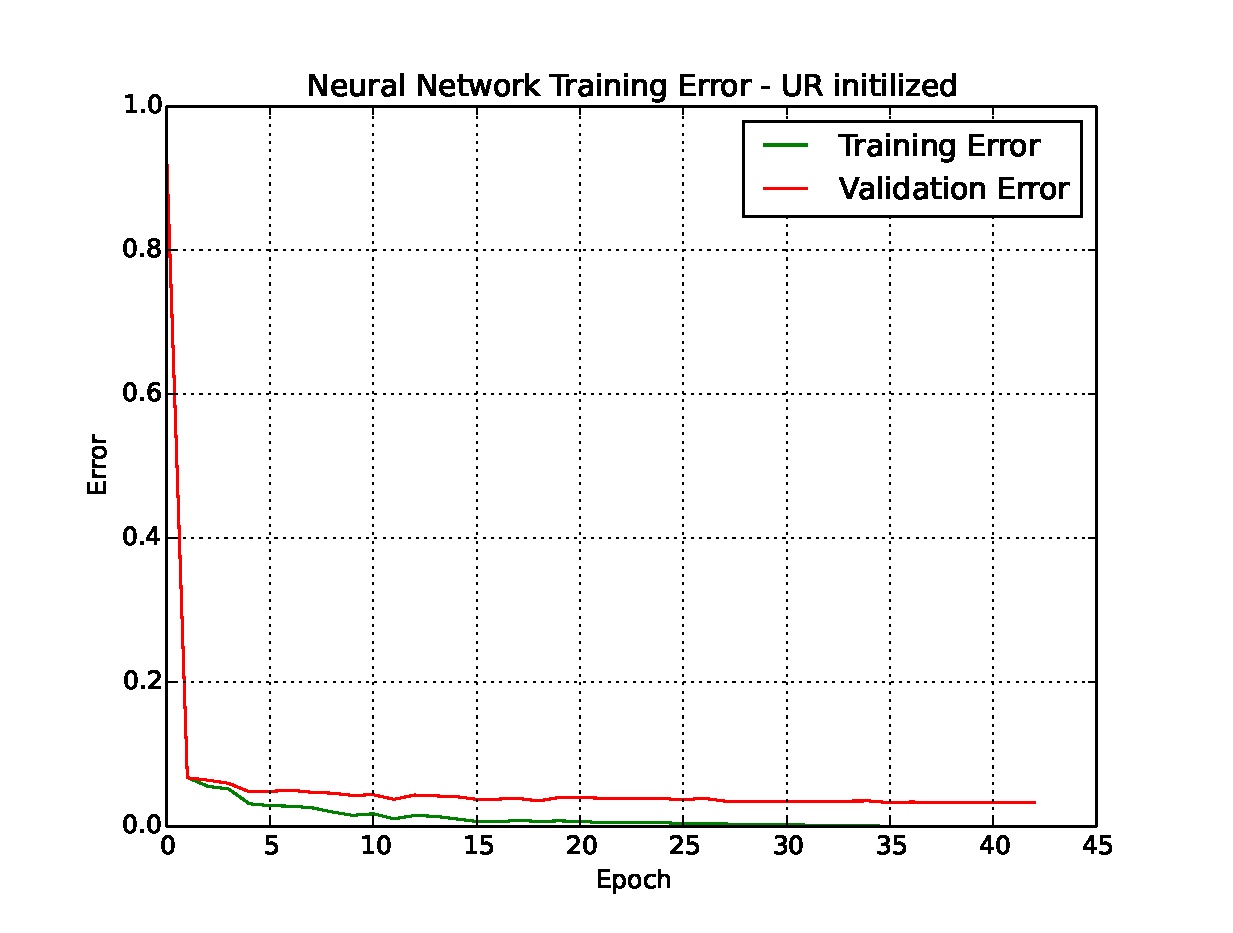
\includegraphics[width=0.8\textwidth,
keepaspectratio]{shallownet_perf.eps} \end{figure}

\begin{figure} \caption{Weight Distribution}
    \medskip
    \small
    L1 maps inputs to hidden layer and L2 maps hidden to output layer. 
    \label{fig:wt_dist} \centering
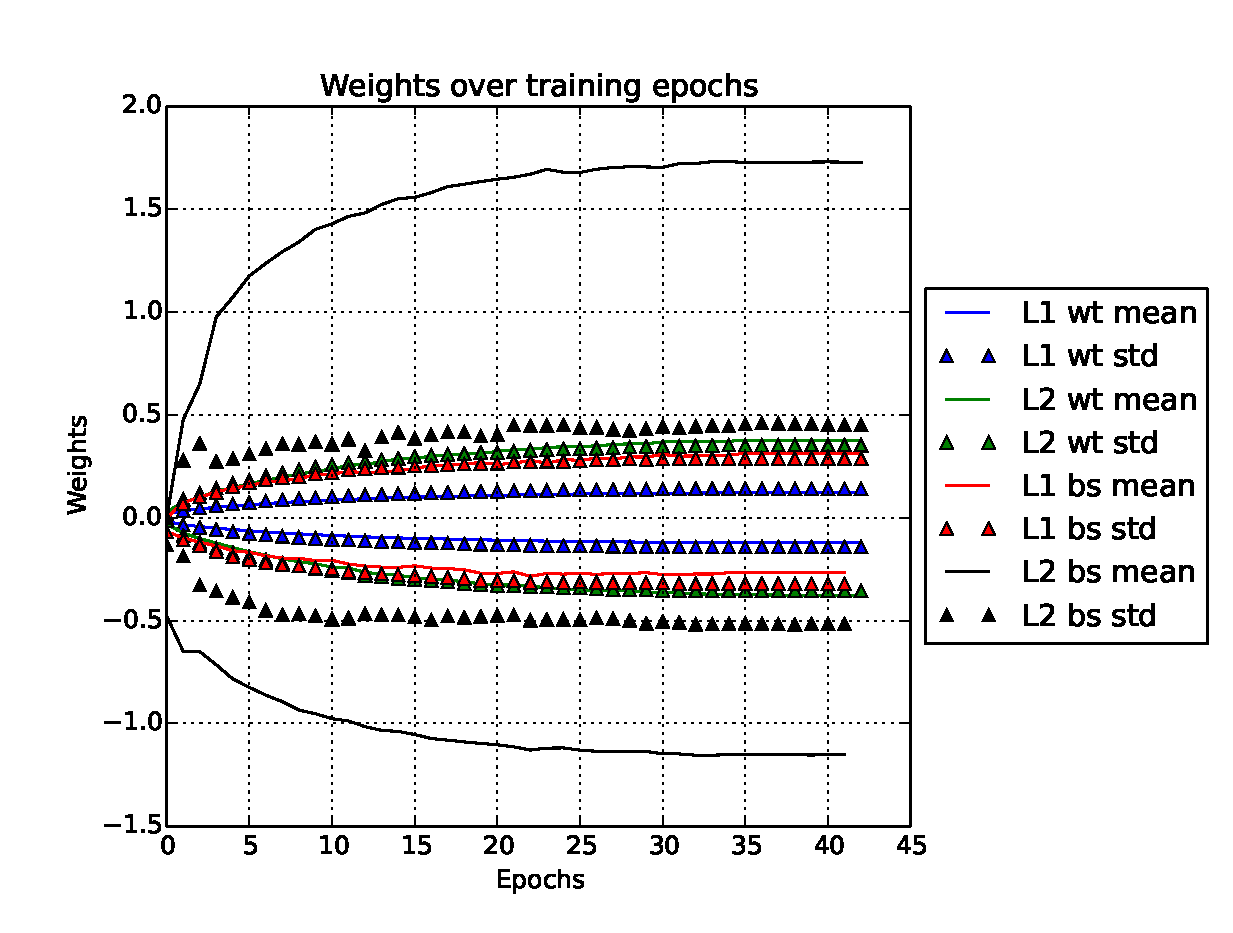
\includegraphics[width=0.95\textwidth, keepaspectratio]{shallownet_weights.eps}
\end{figure}

\begin{figure} \centering \label{fig:actv_dist}
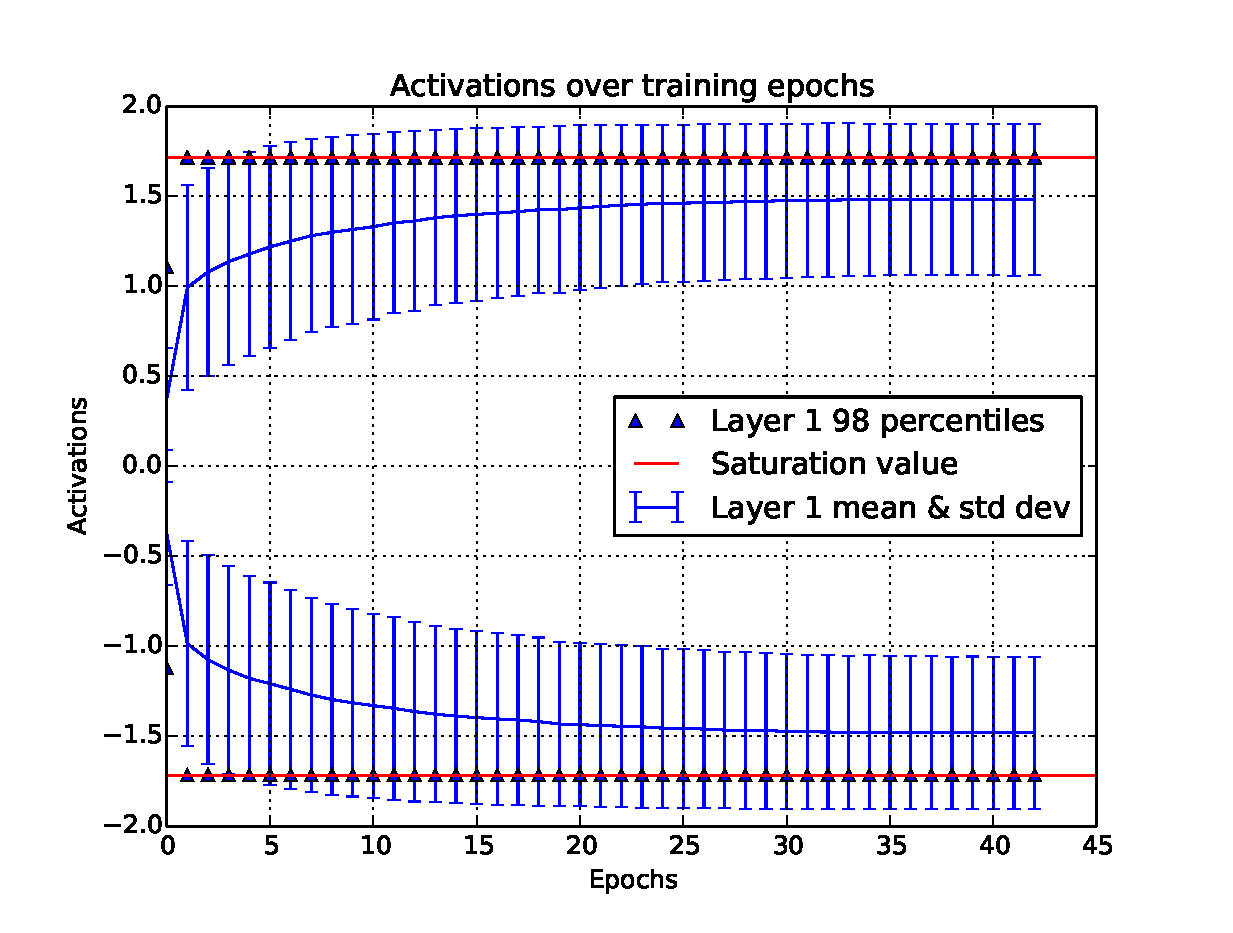
\includegraphics[width=0.8\textwidth, keepaspectratio]{shallownet_actv.eps}
\caption{Layer 1 Activations} \end{figure}


\subsection{Random Features Network} We performed an experiment to determine
the performance of neural network with random (linear and non linear) features.
This is done by keeping the weights and biases of layer $1$ fixed, while
changing only the weights and biases of layer $2$ using Back Propagation. The
weights and biases in layer $2$ are initialized as mentioned in
section~\ref{sec:weight_init} while the weights and biases in layer $1$ are sampled
randomly from a uniform distribution $U[-a, a]$ where $a$ is varied from $0.01$
to $3.0$. The hidden layer is set to have $300$ hidden units. The network is
trained using back propagation for $10$ epochs with a fixed learning rate and
batch size as mentioned in section~\ref{sec:train_method}. The error obtained
on the test set is recorded in table~\ref{tab:terror}. The number of epochs was
fixed to $10$ because the training error did not drop further after the first
epoch. We also did one experiment by choosing the $a=0.6$ such that the mean of
all activations in the hidden layer lies between the linear region of the
activation function and its saturation value, see
figure~\ref{fig:ll_actv_dist}. We also increased the number of hidden units to
$900$. We observed that although the training error dropped below $10\%$ slowly
over $50$ epochs, the validation error did not drop below $10\%$; see
figure~\ref{fig:ll_test_err}. From the observations we think that when the
first hidden layer generates random features activations, the biases mapping
hidden layer to output layer become large in an effort to reduce output error,
while the weights remain small; see figure~\ref{fig:ll_50ep_train_err}.

\begin{table}[H] \centering \begin{tabular}{|c||c|} \hline $a$&$Test Error (\%)$\\
\hline \hline 0.01&8.85\\ 0.035&8.87\\ 0.1&10.72\\ 0.3&12.9\\
0.9&14.88\\ 3.0&15.54\\ \hline \end{tabular} \caption{Random Feature Network
with 300 Hidden Units} \label{tab:terror} \end{table}

\begin{figure}[H]
    \caption{Training and Validation Error}
    \label{fig:ll_test_err}
    \centering
    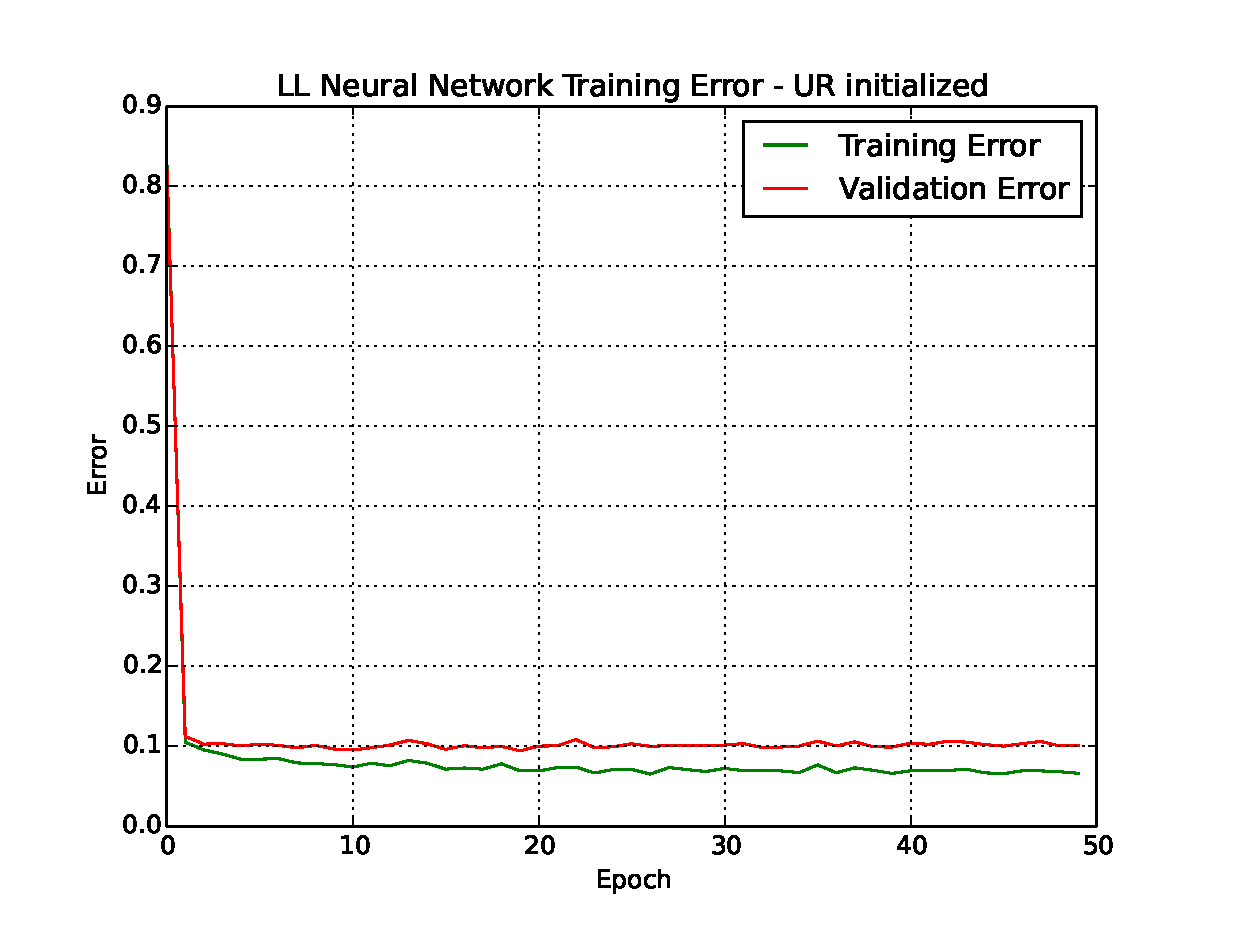
\includegraphics[width=0.8\textwidth,keepaspectratio]{ll_perf.eps}
\end{figure}

\begin{figure}[H]
    \caption{layer 1 activations}
    \label{fig:ll_actv_dist}
    \centering
    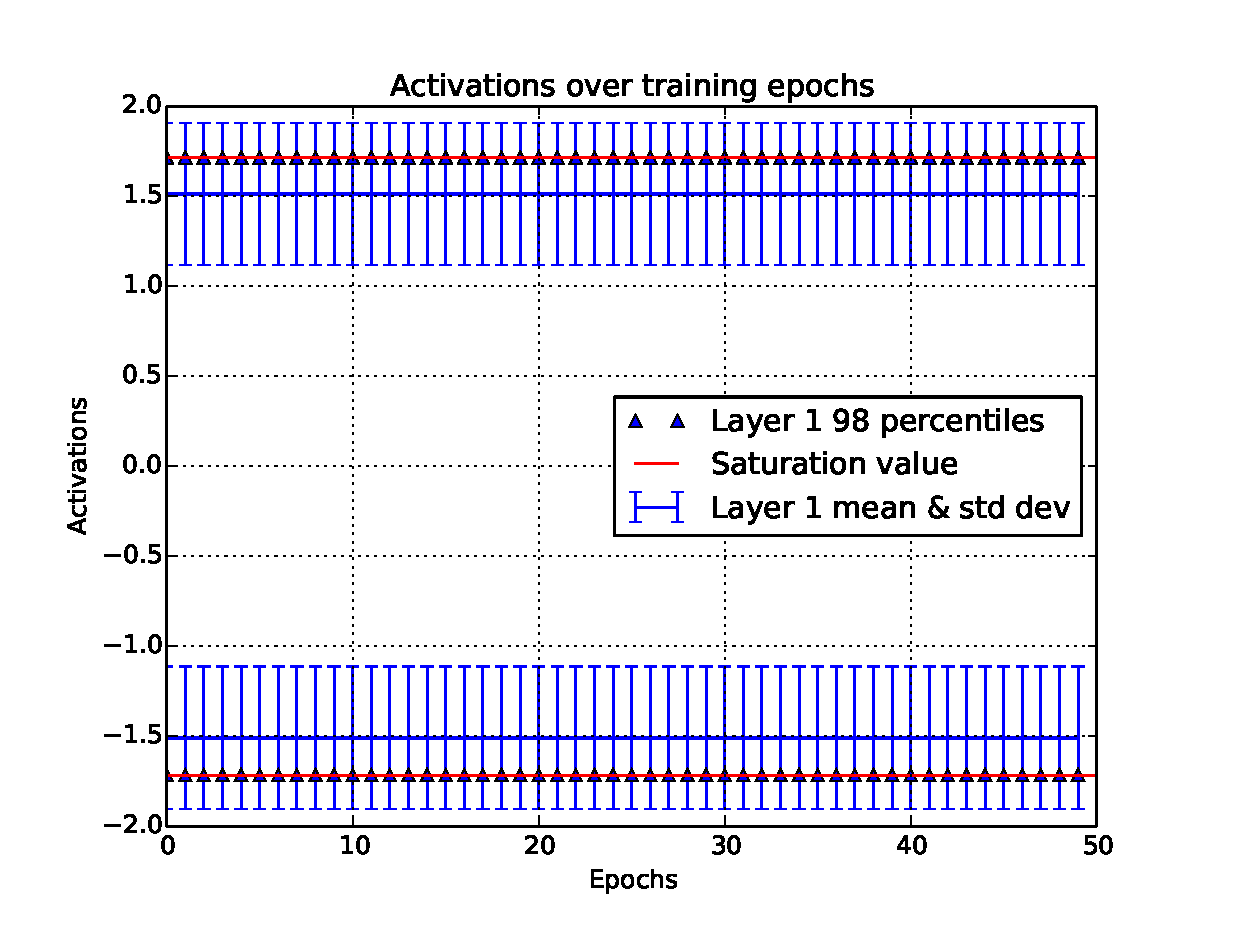
\includegraphics[width=0.8\textwidth,keepaspectratio]{ll_actv.eps}
\end{figure}

\begin{figure}[H]
    \caption{Weight Distribution}
    \medskip
    \small
    L1 maps inputs to hidden layer and L2 maps hidden to output layer. 
    \label{fig:ll_50ep_train_err}
    \centering
    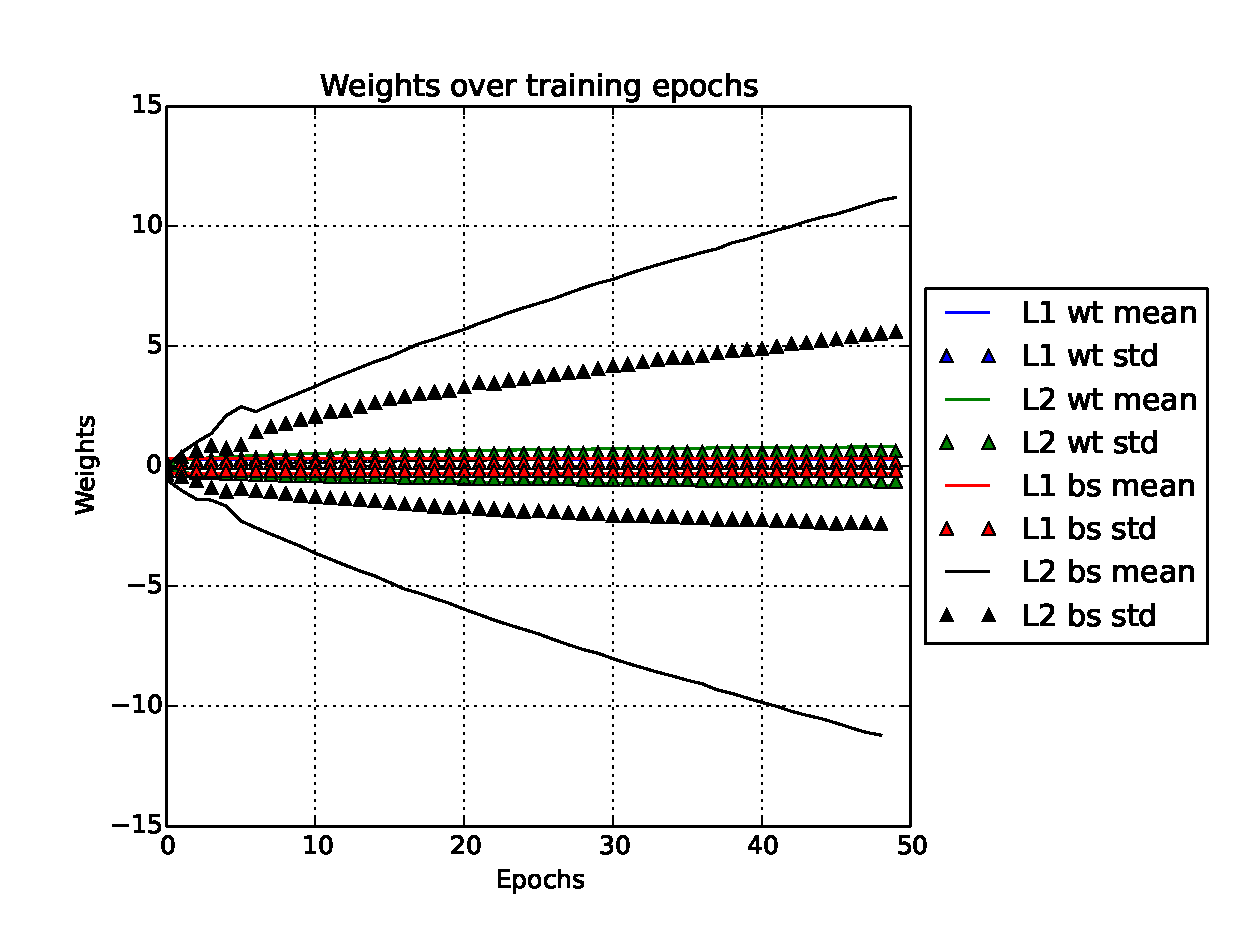
\includegraphics[width=0.8\textwidth,keepaspectratio]{ll_weights_50ep.eps}
\end{figure}

\bibliography{report}{References}
\bibliographystyle{plain}
\end{document}

